% Diagrama de blocos da malha de controle em cascata com feedforward.
% Layout modelo: Figuras/cascata_feedforward.png (linha principal unica,
% feedforward e perturbacao em ruas superiores, realimentacoes em ruas
% inferiores horizontais, dobras ortogonais a 90°).
\documentclass[border=5pt]{standalone}
\usepackage[T1]{fontenc}
\usepackage[utf8]{inputenc}
\usepackage{amsmath}
\usepackage{graphicx}
\usepackage{tikz}
\usetikzlibrary{positioning,arrows.meta,calc}

\begin{document}
\resizebox{175mm}{!}{%
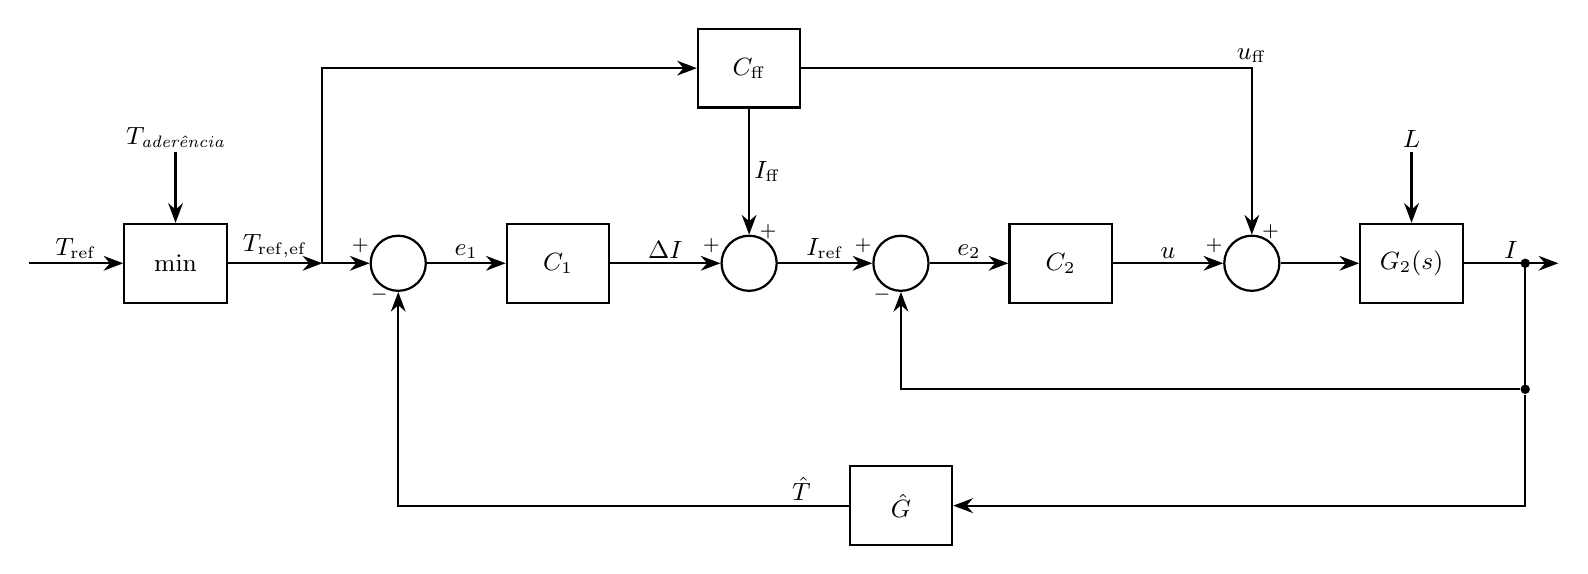
\begin{tikzpicture}[
    font=\small,
    block/.style={draw=black, thick, minimum height=10mm, minimum width=13mm, inner sep=2pt},
    sum/.style={circle, draw=black, thick, minimum size=7mm, inner sep=0pt},
    sign/.style={font=\scriptsize, inner sep=1pt},
    sig/.style={font=\itshape\small, inner sep=1.5pt},
    arrow/.style={-{Stealth[length=2.5mm]}, thick}
  ]

  % ================= Linha principal (y = 0) =================
  \node[block] (min) {min};
  \node[sig, above=9mm of min] (tadh) {$T_{\text{ader\^encia}}$};
  \draw[arrow] (tadh.south) -- (min.north);
  \draw[arrow] ($(min.west)+(-12mm,0)$) -- node[sig, above] {$T_{\mathrm{ref}}$} (min.west);

  \coordinate[right=12mm of min] (split);
  \draw[arrow] (min.east) -- node[sig, above] {$T_{\mathrm{ref,ef}}$} (split);

  % Somador 1: malha mestra (+/-)
  \node[sum, right=18mm of min] (s1) {};
  \node[sign] at ($(s1.center)+(-4.8mm,2.2mm)$) {$+$};
  \node[sign] at ($(s1.center)+(-2.4mm,-4.0mm)$) {$-$};
  \draw[arrow] (split) -- (s1.west);

  \node[block, right=10mm of s1] (c1) {$C_1$};
  \draw[arrow] (s1.east) -- node[sig, above] {$e_1$} (c1.west);

  % Somador 2 (+/+): Delta I + I_ff (I_ff entra por cima)
  \node[sum, right=14mm of c1] (s2) {};
  \node[sign] at ($(s2.center)+(-4.8mm,2.2mm)$) {$+$};
  \node[sign] at ($(s2.center)+(2.4mm,4.0mm)$) {$+$};
  \draw[arrow] (c1.east) -- node[sig, above] {$\Delta I$} (s2.west);

  % Somador 3: malha escrava (+/-)
  \node[sum, right=12mm of s2] (s3) {};
  \node[sign] at ($(s3.center)+(-4.8mm,2.2mm)$) {$+$};
  \node[sign] at ($(s3.center)+(-2.4mm,-4.0mm)$) {$-$};
  \draw[arrow] (s2.east) -- node[sig, above] {$I_{\mathrm{ref}}$} (s3.west);

  \node[block, right=10mm of s3] (c2) {$C_2$};
  \draw[arrow] (s3.east) -- node[sig, above] {$e_2$} (c2.west);

  % Somador 4 (+/+): u + u_ff (u_ff entra por cima)
  \node[sum, right=14mm of c2] (s4) {};
  \node[sign] at ($(s4.center)+(-4.8mm,2.2mm)$) {$+$};
  \node[sign] at ($(s4.center)+(2.4mm,4.0mm)$) {$+$};
  \draw[arrow] (c2.east) -- node[sig, above] {$u$} (s4.west);

  \node[block, right=10mm of s4] (g2) {$G_2(s)$};
  \draw[arrow] (s4.east) -- (g2.west);
  \node[sig, above=9mm of g2] (l) {$L$};
  \draw[arrow] (l.south) -- (g2.north);

  \coordinate[right=12mm of g2] (outI);
  \coordinate (itap) at ($(g2.east)!0.65!(outI)$);
  \draw[arrow] (g2.east) -- node[sig, above] {$I$} (outI);
  \node[circle, fill=black, inner sep=1.2pt] at (itap) {};

  % ============ Feedforward (rua superior, como o FFC da referencia) ====
  \node[block, above=16mm of s2] (cff) {$C_{\mathrm{ff}}$};
  \draw[arrow] (split) |- (cff.west);

  % I_ff desce diretamente ao somador 2
  \draw[arrow] (cff.south) -- node[sig, right] {$I_{\mathrm{ff}}$} (s2.north);

  % u_ff segue na rua superior e desce ao somador 4
  \draw[arrow] (cff.east) -| node[sig, above, pos=0.5] {$u_{\mathrm{ff}}$} (s4.north);

  % ======== Realimentacoes: tronco unico a partir do no I ==============
  % Uma unica linha desce do no I; num ponto de derivacao (no preto) na
  % rua intermediaria (y = -16mm) o sinal se divide: um ramo segue pela
  % rua intermediaria e sobe ao somador 3 (malha escrava); o outro continua
  % descendo e entra pelo lado DIREITO do G-hat (malha mestra).
  % Estimador: bloco horizontal centrado abaixo da linha principal,
  % fluxo direita -> esquerda; \hat{T} sai pela esquerda e retorna pela
  % rua inferior ate o somador 1.
  \node[block, below=22mm of s3] (ghat) {$\hat{G}$};
  \draw[thick] (itap) -- ($(itap)+(0,-16mm)$);
  \node[circle, fill=black, inner sep=1.2pt] (idot) at ($(itap)+(0,-16mm)$) {};
  \draw[arrow] (idot) -| (s3.south);
  \draw[arrow] (idot) |- (ghat.east);
  \draw[arrow] (ghat.west) -- ++(-6mm,0) node[sig, above] {$\hat{T}$} -| (s1.south);

\end{tikzpicture}}
\end{document}
